\subsection{Melting temperature of short hairpins}

Another test of the model with regard to hairpin formation is to see if it can reproduce the correct critical temperatures for short hairpins. We consider a small class of hairpins that have received extensive experimental attention by Vallone \etal \cite{vallone1999melting}.

This class of hairpin sequences are composed of of a loop part consisting of four monomers with the same base type, this loop part is then flanked on either side by two monomers that form complementary pairs. At the end of each strand, there is a fixed sequence of four complementary monomers (CCTA and TAGG), which brings the total number of monomers to sixteen.

We selected two specific sequences, comprised of an adenine loop and with variable base sequences equal to TT/AA and TG/CA. The ionic strength of the world was set to 115\,mM, mimicking the experimental setup in \cite{vallone1999melting}.

We allowed the strand to fully equilibrate for 0.5\,$\mu$s, after which we tracked and averaged the number of base pair bonds in time. As before, a base pair is considered `bound' if its base pairing potential is less than $-\varepsilon / 10$.


\begin{figure}[htb]
       \begin{center}
               \scalebox{0.9}{
                        \nonstopmode
                        % GNUPLOT: LaTeX picture with Postscript
\begingroup
  \makeatletter
  \providecommand\color[2][]{%
    \GenericError{(gnuplot) \space\space\space\@spaces}{%
      Package color not loaded in conjunction with
      terminal option `colourtext'%
    }{See the gnuplot documentation for explanation.%
    }{Either use 'blacktext' in gnuplot or load the package
      color.sty in LaTeX.}%
    \renewcommand\color[2][]{}%
  }%
  \providecommand\includegraphics[2][]{%
    \GenericError{(gnuplot) \space\space\space\@spaces}{%
      Package graphicx or graphics not loaded%
    }{See the gnuplot documentation for explanation.%
    }{The gnuplot epslatex terminal needs graphicx.sty or graphics.sty.}%
    \renewcommand\includegraphics[2][]{}%
  }%
  \providecommand\rotatebox[2]{#2}%
  \@ifundefined{ifGPcolor}{%
    \newif\ifGPcolor
    \GPcolortrue
  }{}%
  \@ifundefined{ifGPblacktext}{%
    \newif\ifGPblacktext
    \GPblacktexttrue
  }{}%
  % define a \g@addto@macro without @ in the name:
  \let\gplgaddtomacro\g@addto@macro
  % define empty templates for all commands taking text:
  \gdef\gplbacktext{}%
  \gdef\gplfronttext{}%
  \makeatother
  \ifGPblacktext
    % no textcolor at all
    \def\colorrgb#1{}%
    \def\colorgray#1{}%
  \else
    % gray or color?
    \ifGPcolor
      \def\colorrgb#1{\color[rgb]{#1}}%
      \def\colorgray#1{\color[gray]{#1}}%
      \expandafter\def\csname LTw\endcsname{\color{white}}%
      \expandafter\def\csname LTb\endcsname{\color{black}}%
      \expandafter\def\csname LTa\endcsname{\color{black}}%
      \expandafter\def\csname LT0\endcsname{\color[rgb]{1,0,0}}%
      \expandafter\def\csname LT1\endcsname{\color[rgb]{0,1,0}}%
      \expandafter\def\csname LT2\endcsname{\color[rgb]{0,0,1}}%
      \expandafter\def\csname LT3\endcsname{\color[rgb]{1,0,1}}%
      \expandafter\def\csname LT4\endcsname{\color[rgb]{0,1,1}}%
      \expandafter\def\csname LT5\endcsname{\color[rgb]{1,1,0}}%
      \expandafter\def\csname LT6\endcsname{\color[rgb]{0,0,0}}%
      \expandafter\def\csname LT7\endcsname{\color[rgb]{1,0.3,0}}%
      \expandafter\def\csname LT8\endcsname{\color[rgb]{0.5,0.5,0.5}}%
    \else
      % gray
      \def\colorrgb#1{\color{black}}%
      \def\colorgray#1{\color[gray]{#1}}%
      \expandafter\def\csname LTw\endcsname{\color{white}}%
      \expandafter\def\csname LTb\endcsname{\color{black}}%
      \expandafter\def\csname LTa\endcsname{\color{black}}%
      \expandafter\def\csname LT0\endcsname{\color{black}}%
      \expandafter\def\csname LT1\endcsname{\color{black}}%
      \expandafter\def\csname LT2\endcsname{\color{black}}%
      \expandafter\def\csname LT3\endcsname{\color{black}}%
      \expandafter\def\csname LT4\endcsname{\color{black}}%
      \expandafter\def\csname LT5\endcsname{\color{black}}%
      \expandafter\def\csname LT6\endcsname{\color{black}}%
      \expandafter\def\csname LT7\endcsname{\color{black}}%
      \expandafter\def\csname LT8\endcsname{\color{black}}%
    \fi
  \fi
  \setlength{\unitlength}{0.0500bp}%
  \begin{picture}(6720.00,4800.00)%
    \gplgaddtomacro\gplbacktext{%
      \colorrgb{0.00,0.00,0.00}%
      \put(741,528){\makebox(0,0)[r]{\strut{}0}}%
      \colorrgb{0.00,0.00,0.00}%
      \put(741,1310){\makebox(0,0)[r]{\strut{}0.2}}%
      \colorrgb{0.00,0.00,0.00}%
      \put(741,2092){\makebox(0,0)[r]{\strut{}0.4}}%
      \colorrgb{0.00,0.00,0.00}%
      \put(741,2875){\makebox(0,0)[r]{\strut{}0.6}}%
      \colorrgb{0.00,0.00,0.00}%
      \put(741,3657){\makebox(0,0)[r]{\strut{}0.8}}%
      \colorrgb{0.00,0.00,0.00}%
      \put(741,4439){\makebox(0,0)[r]{\strut{}1}}%
      \colorrgb{0.00,0.00,0.00}%
      \put(873,308){\makebox(0,0){\strut{}0}}%
      \colorrgb{0.00,0.00,0.00}%
      \put(1915,308){\makebox(0,0){\strut{}20}}%
      \colorrgb{0.00,0.00,0.00}%
      \put(2956,308){\makebox(0,0){\strut{}40}}%
      \colorrgb{0.00,0.00,0.00}%
      \put(3998,308){\makebox(0,0){\strut{}60}}%
      \colorrgb{0.00,0.00,0.00}%
      \put(5039,308){\makebox(0,0){\strut{}80}}%
      \colorrgb{0.00,0.00,0.00}%
      \put(6081,308){\makebox(0,0){\strut{}100}}%
      \colorrgb{0.00,0.00,0.00}%
      \put(103,2483){\rotatebox{90}{\makebox(0,0){\strut{}\rule{0pt}{-1.5cm}Fraction of bound base pairs in the stem}}}%
      \colorrgb{0.00,0.00,0.00}%
      \put(3477,-22){\makebox(0,0){\strut{}Temperature ($\degree$C)}}%
    }%
    \gplgaddtomacro\gplfronttext{%
    }%
    \gplbacktext
    \put(0,0){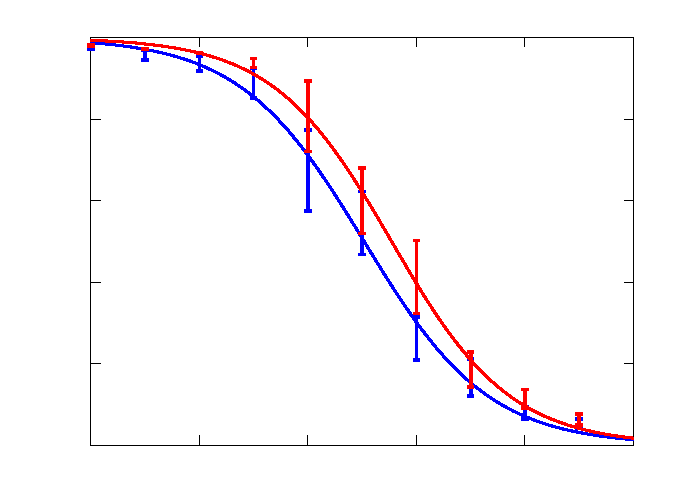
\includegraphics{images/meltingTemperature}}%
    \gplfronttext
  \end{picture}%
\endgroup

                        \errorstopmode
                        \rule[-0.5cm]{0cm}{0cm}}
                \caption{Melting transition of two DNA hairpins: 3'CCTA\textbf{TT}AAAA\textbf{AA}TAGG5' (blue) and 3'CCTA\textbf{TG}AAAA\textbf{CA}TAGG5' (red). The simulation is performed at an ionic strenght of 115\,mM, compatible with \cite{vallone1999melting}. The data is fitted by a tanh function, giving a critical temperature of $(55.3 \pm 0.5)\degree$C and $(50.3 \pm 0.8)\degree$C for the red (TG/CA) and blue (TT/AA) curve, respectively.}
                \label{meltingTemperature}
        \end{center}
\end{figure}



The simulations were run for a range of temperatures between 0$\degree$C and 90$\degree$C. At each temperature, a total of at least 8 simulation runs was averaged.
The resulting curves are shown in Figure \ref{meltingTemperature}. We find critical temperatures (defined as the temperature where the average fraction of bound base pairs in the stem equals 50\%) of $(55.4 \pm 0.5)\degree$C for the TG/CA sequence, and $(50.3 \pm 0.8)\degree$C for the TT/AA sequence. A lower critical temperature for this latter sequence is to be expected, as the base pairing interaction between A/T pairs is less than that between G/C pairs.

The experimental values reported by Vallone \etal\ are $(35 \pm 1)\degree$C for the TT/AA sequence and $(55.5 \pm 0.3)\degree$C for the TG/CA sequence.\cite{vallone1999melting}. The simulated value for the TG/CA sequence is spot on, but the value for the TT/AA sequence is off by quite a bit.

The reason for this discrepancy could be because the model was initially fitted to reproduce experimental values for long base pair sequences. It also ignores hydrodynamic interactions, which are shown to be of significant importance in small strands and loops \cite{kuznetsov2001semiflexible, shen2001loop, vallone1999melting}.

Lastly we remark that the rescaling of the base pairing interaction by Florescu and Joyeux is essential to get the correct order of magnitude.
Indeed, using the interaction constants of the original Knotts model ($\epsAT = 2.77$\,kcal/mol and $\epsGC = 4.16$\,kcal/mol), but keeping the base pairing interaction between the `correctly matching' base pairs on the hairpin only (as per \cite{florescu2011thermal}) leads to very unphysical results. This is shown in Figure \ref{meltingTemperatureKnotts}. 

In light of this large discrepancy generated by the rather modest change in base pair interaction strength, the deviation of the melting temperature for the TT/AA curve in Figure \ref{meltingTemperature} does not seem so bad.

\begin{figure}[htb]
       \begin{center}
               \scalebox{0.9}{
                        \nonstopmode
                        % GNUPLOT: LaTeX picture with Postscript
\begingroup
  \makeatletter
  \providecommand\color[2][]{%
    \GenericError{(gnuplot) \space\space\space\@spaces}{%
      Package color not loaded in conjunction with
      terminal option `colourtext'%
    }{See the gnuplot documentation for explanation.%
    }{Either use 'blacktext' in gnuplot or load the package
      color.sty in LaTeX.}%
    \renewcommand\color[2][]{}%
  }%
  \providecommand\includegraphics[2][]{%
    \GenericError{(gnuplot) \space\space\space\@spaces}{%
      Package graphicx or graphics not loaded%
    }{See the gnuplot documentation for explanation.%
    }{The gnuplot epslatex terminal needs graphicx.sty or graphics.sty.}%
    \renewcommand\includegraphics[2][]{}%
  }%
  \providecommand\rotatebox[2]{#2}%
  \@ifundefined{ifGPcolor}{%
    \newif\ifGPcolor
    \GPcolortrue
  }{}%
  \@ifundefined{ifGPblacktext}{%
    \newif\ifGPblacktext
    \GPblacktexttrue
  }{}%
  % define a \g@addto@macro without @ in the name:
  \let\gplgaddtomacro\g@addto@macro
  % define empty templates for all commands taking text:
  \gdef\gplbacktext{}%
  \gdef\gplfronttext{}%
  \makeatother
  \ifGPblacktext
    % no textcolor at all
    \def\colorrgb#1{}%
    \def\colorgray#1{}%
  \else
    % gray or color?
    \ifGPcolor
      \def\colorrgb#1{\color[rgb]{#1}}%
      \def\colorgray#1{\color[gray]{#1}}%
      \expandafter\def\csname LTw\endcsname{\color{white}}%
      \expandafter\def\csname LTb\endcsname{\color{black}}%
      \expandafter\def\csname LTa\endcsname{\color{black}}%
      \expandafter\def\csname LT0\endcsname{\color[rgb]{1,0,0}}%
      \expandafter\def\csname LT1\endcsname{\color[rgb]{0,1,0}}%
      \expandafter\def\csname LT2\endcsname{\color[rgb]{0,0,1}}%
      \expandafter\def\csname LT3\endcsname{\color[rgb]{1,0,1}}%
      \expandafter\def\csname LT4\endcsname{\color[rgb]{0,1,1}}%
      \expandafter\def\csname LT5\endcsname{\color[rgb]{1,1,0}}%
      \expandafter\def\csname LT6\endcsname{\color[rgb]{0,0,0}}%
      \expandafter\def\csname LT7\endcsname{\color[rgb]{1,0.3,0}}%
      \expandafter\def\csname LT8\endcsname{\color[rgb]{0.5,0.5,0.5}}%
    \else
      % gray
      \def\colorrgb#1{\color{black}}%
      \def\colorgray#1{\color[gray]{#1}}%
      \expandafter\def\csname LTw\endcsname{\color{white}}%
      \expandafter\def\csname LTb\endcsname{\color{black}}%
      \expandafter\def\csname LTa\endcsname{\color{black}}%
      \expandafter\def\csname LT0\endcsname{\color{black}}%
      \expandafter\def\csname LT1\endcsname{\color{black}}%
      \expandafter\def\csname LT2\endcsname{\color{black}}%
      \expandafter\def\csname LT3\endcsname{\color{black}}%
      \expandafter\def\csname LT4\endcsname{\color{black}}%
      \expandafter\def\csname LT5\endcsname{\color{black}}%
      \expandafter\def\csname LT6\endcsname{\color{black}}%
      \expandafter\def\csname LT7\endcsname{\color{black}}%
      \expandafter\def\csname LT8\endcsname{\color{black}}%
    \fi
  \fi
  \setlength{\unitlength}{0.0500bp}%
  \begin{picture}(6720.00,4800.00)%
    \gplgaddtomacro\gplbacktext{%
      \colorrgb{0.00,0.00,0.00}%
      \put(741,528){\makebox(0,0)[r]{\strut{}0}}%
      \colorrgb{0.00,0.00,0.00}%
      \put(741,1087){\makebox(0,0)[r]{\strut{}0.1}}%
      \colorrgb{0.00,0.00,0.00}%
      \put(741,1645){\makebox(0,0)[r]{\strut{}0.2}}%
      \colorrgb{0.00,0.00,0.00}%
      \put(741,2204){\makebox(0,0)[r]{\strut{}0.3}}%
      \colorrgb{0.00,0.00,0.00}%
      \put(741,2763){\makebox(0,0)[r]{\strut{}0.4}}%
      \colorrgb{0.00,0.00,0.00}%
      \put(741,3322){\makebox(0,0)[r]{\strut{}0.5}}%
      \colorrgb{0.00,0.00,0.00}%
      \put(741,3880){\makebox(0,0)[r]{\strut{}0.6}}%
      \colorrgb{0.00,0.00,0.00}%
      \put(741,4439){\makebox(0,0)[r]{\strut{}0.7}}%
      \colorrgb{0.00,0.00,0.00}%
      \put(873,308){\makebox(0,0){\strut{}0}}%
      \colorrgb{0.00,0.00,0.00}%
      \put(1915,308){\makebox(0,0){\strut{}20}}%
      \colorrgb{0.00,0.00,0.00}%
      \put(2956,308){\makebox(0,0){\strut{}40}}%
      \colorrgb{0.00,0.00,0.00}%
      \put(3998,308){\makebox(0,0){\strut{}60}}%
      \colorrgb{0.00,0.00,0.00}%
      \put(5039,308){\makebox(0,0){\strut{}80}}%
      \colorrgb{0.00,0.00,0.00}%
      \put(6081,308){\makebox(0,0){\strut{}100}}%
      \colorrgb{0.00,0.00,0.00}%
      \put(103,2483){\rotatebox{90}{\makebox(0,0){\strut{}\rule{0pt}{-1.5cm}Fraction of bound base pairs in the stem}}}%
      \colorrgb{0.00,0.00,0.00}%
      \put(3477,-22){\makebox(0,0){\strut{}Temperature ($\degree$C)}}%
    }%
    \gplgaddtomacro\gplfronttext{%
    }%
    \gplbacktext
    \put(0,0){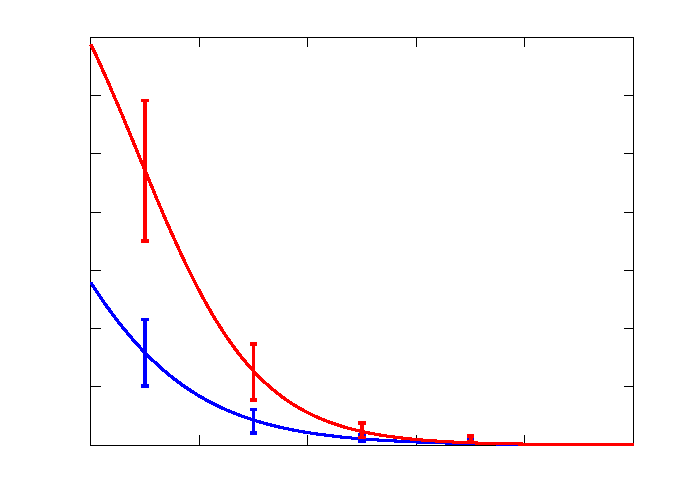
\includegraphics{images/meltingTemperatureKnotts}}%
    \gplfronttext
  \end{picture}%
\endgroup

                        \errorstopmode
                        \rule[-0.5cm]{0cm}{0cm}}
                \caption{Melting transition of the same DNA hairpin sequences as in figure \ref{meltingTemperature}, but with base pairing interaction constants as per Knotts \etal \cite{knotts2007coarse}, while keeping the interaction btween matching hairpin base pairs only. This leads to very unphysical melting temperatures of ($8.7 \pm 0.3)\degree$C for the red (TG/CA) curve and ($-13 \pm 2)\degree$C for the blue (TT/AA) curve.}
                \label{meltingTemperatureKnotts}
        \end{center}
\end{figure}


